\section{System Study and Analysis }

\subsection{Existing System }
\paragraph{}Current online learning systems are often built on fragmented data distributed across multiple platforms and locations. Students often face difficulties accessing general education content. They may need to browse multiple websites, apps, or physical resources to find relevant information, resulting in inconsistent learning. Additionally, the current system may not have interactive, self-selecting, and immediate feedback strategies, which may limit the effectiveness of the learning process. Overall, the current system may not be able to meet the changing needs and expectations of students in terms of accessibility, participation and flexibility in personal learning styles.

\subsection{Proposed System}
\paragraph{}The proposed system, Query Quest - Edu, aims to transform the current online education system by providing simple and comprehensive learning. Query Quest - Edu will provide a central place where users can access different educational content, unlike the resources of the current system. The platform will include a variety of content that will allow students to access resources based on their interests and learning goals. Focusing on user interaction and integration, Query Quest - Edu will provide interactive and practical options to enhance learning for all users. Through personalized recommendations and appropriate design, Query Quest - Edu aims to help students take control of their learning and realize their full potential.

\subsection{Feasibility System}
\paragraph{}Query Quest - Edu's study on the feasibility and effectiveness of implementing the planning process. It takes into account many factors such as work, work and productivity to determine efficiency and sustainability.

\begin{itemize}
    

\item Technical Feasibility: This aspect evaluates whether the proposed process can be developed using existing tools and resources. It evaluates features such as compatibility between software tools, data management, and programming languages needed for development. Additionally, technical feasibility checks the scalability and performance of the system to meet future growth and user needs.

\item Economic Feasibility: Economic feasibility analyzes the cost effectiveness of the design and management of the planning process. It takes into account things like construction costs, hardware and software costs, operating costs, and capital gains. Business feasibility also examines the project's return on investment (ROI) and financial value over time.

\item Operational Feasibility: Operational Feasibility measures the effectiveness of using the proposed system in an organization or user community. It considers factors such as user acceptance, training needs, operational planning, and potential impact on existing operations and processes. Functionality also measures the ease of maintaining, updating, and supporting a system on an ongoing basis.
\end{itemize}

\paragraph{}This research provides information on the technical, economic and operational aspects of the project, ultimately contributing to the success and long-term sustainability of the project.


\newpage


















\section{Data Flow }
% \begin{figure}[h!]
%     \centering
%      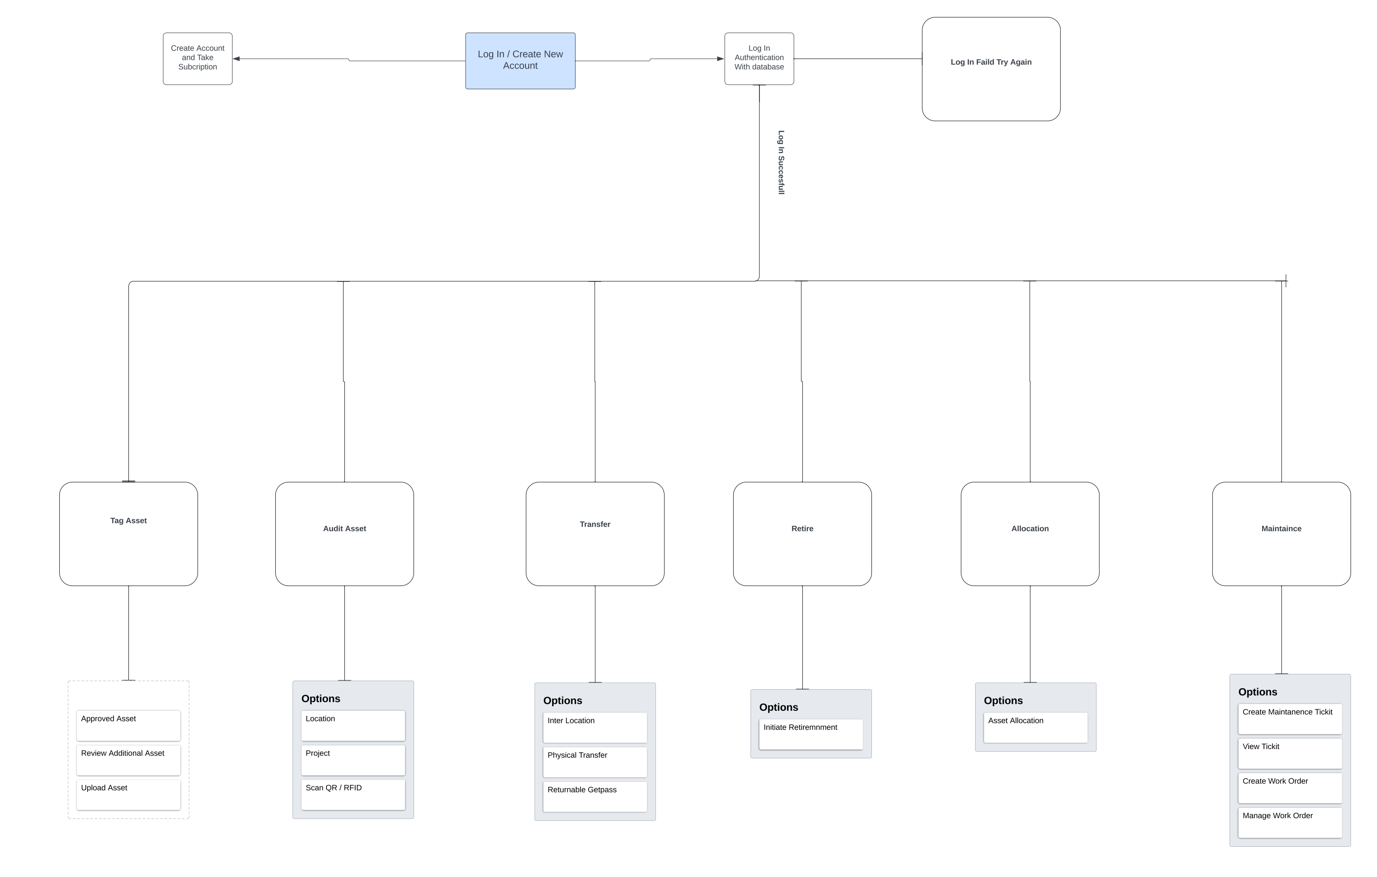
\includegraphics[scale=0.6]{save.png}  
% \end{figure}


% % New text insertion after the figure
% The diagram appears to show a high-level overview of a cloud-based warehouse management system (WMS). The main components of the system include a supervisor's room, a main warehouse, a cloud database, individual warehouses, RFID readers, mobile apps, and information sharing. The system uses RFID readers to track the location of goods in the warehouse, and this information is stored in the cloud database. The supervisor can use the information in the cloud database to monitor the warehouse operation and make sure that it is running smoothly. The system can be used to improve the efficiency and accuracy of warehouse operations.





% \newpage










\section{System Design }
% \subsection{File Upload Page}
% \begin{figure}[h!]
%     \centering
%     \includegraphics[scale=0.4]{uplodede.png}  
%      \caption{\textbf{Upload Page (Before Asset File Upload)}}
% \end{figure}

% \begin{figure}[h!]
%     \centering
%     \includegraphics[scale=0.4]{uploded.png}  
%      \caption{\textbf{Upload Page (After Asset File Upload)}}
% \end{figure}
% \vspace{0.5cm}

% \begin{enumerate}
%   \item Its an asset file upload page(Excel File).
%   \item Here user upload a assets with their description in the form of columns, the user can map a their file columns and columns inside a tables to add all upload all assets in bulk.
% \end{enumerate}

% \newpage
% \subsection{Home Page}
% \begin{figure}[h!]
%     \centering
%     \includegraphics[scale=0.4]{1 (1).jpeg}  
%      \caption{\textbf{Home Page}}
% \end{figure}

% \vspace{0.5cm}

% \begin{enumerate}
%   \item It's a home page of our mobile application and its contains a various buttons  to access all components for asset tracking.
%   \item Some examples of buttons like Tag asset gives access to asset tagging component, Transfer buttons Gives access to Transfer Asset Component etc
% \end{enumerate}
% \newpage
% \subsection{Topic}
% \begin{figure}[h!]
%     \centering
%      \includegraphics[scale=0.4]{1 (2).jpeg} 
%      \caption{\textbf{Asset Tagging Page}}
% \end{figure}
% \vspace{0.5cm}

% \begin{enumerate}
%   \item Its an asset tagging component,Used for tagging of asset.
%   \item In this component we can upload photo and also we can scan the asset for its tagging.
% \end{enumerate}
% \newpage
% \subsection{Topic}
% \begin{figure}[h!]
%     \centering
%      \includegraphics[scale=0.4]{transfer.jpeg} 
%       \caption{\textbf{Transfer Page}}
% \end{figure}
% \vspace{0.5cm}

% \begin{enumerate}
%   \item Transfer page is to track the location of asset.
%   \item Using this component we can track the asset like we can see the exact location of asset, we can check is this asset inside the organization or someone use this asset from home for WFH.
% \end{enumerate}
% \newpage
% \subsection{Topic}
% \begin{figure}[h!]
%     \centering
%      \includegraphics[scale=0.4]{audit.jpeg} 
%       \caption{\textbf{Audit Page}}
% \end{figure}
% \vspace{0.5cm}

% \begin{enumerate}
%   \item Using audit component we check the assets used by the branch and project.
%   \item On this component we see the total summary of assets used in particular project and location.
% \end{enumerate}
% \newpage
% \subsection{Topic}
% \begin{figure}[h!]
%     \centering
%      \includegraphics[scale=0.4]{retire.jpeg} 
%       \caption{\textbf{Retire Page}}
% \end{figure}
% \vspace{0.5cm}

% \begin{enumerate}
%   \item Using the retire component we check the life of asset and we can generate its retirement ticket.
%   \item Here we can add a retirement status to known the process of retirement.
% \end{enumerate}
% \newpage

% \subsection{Topic}
% \begin{figure}[h!]
%     \centering
%      \includegraphics[scale=0.4]{1 (5).jpeg} 
%       \caption{\textbf{Allocation Page}}
% \end{figure}
% \vspace{0.5cm}

% \begin{enumerate}
%   \item Using this allocation component we can allocate the asset to any person or project.
%   \item After the allocation we check the is we need to transfer this asset or not.
% \end{enumerate}
 
% \newpage
% \subsection{Topic}

% \begin{figure}[h!]
%     \centering
%      \includegraphics[scale=0.4]{1 (9).jpeg}
%       \caption{\textbf{Maintenance Page}}
% \end{figure}
%  \vspace{0.5cm}

% \begin{enumerate}
%   \item In this maintenance component we add a all feature to  the maintenance of asset.
%   \item In that we create a Maintenance Ticket, View created ticket,Create work order and manage work order.
% \end{enumerate}



